% AlphaOrchestra business plan converted from DOCX.
% Formatting-only LaTeX version; source content is preserved.
\documentclass[12pt,a4paper]{ctexart}

\usepackage[a4paper,top=2.6cm,bottom=2.6cm,left=2.8cm,right=2.8cm]{geometry}
\usepackage{fontspec}
\usepackage{amsmath,amssymb}
\usepackage{unicode-math}
\usepackage{xcolor}
\usepackage{graphicx}
\usepackage{float}
\usepackage{longtable,booktabs,array}
\usepackage{etoolbox}
\usepackage{calc}
\usepackage{tabularx}
\usepackage{ragged2e}
\usepackage{enumitem}
\usepackage{titlesec}
\usepackage{fancyhdr}
\usepackage{setspace}
\usepackage{microtype}
\usepackage{newunicodechar}
\usepackage{xurl}
\usepackage[hidelinks]{hyperref}
\usepackage{bookmark}
\setcounter{secnumdepth}{-\maxdimen}

\IfFontExistsTF{Times New Roman}{\setmainfont{Times New Roman}}{\setmainfont{TeX Gyre Termes}}
\IfFontExistsTF{SimSun}{\setCJKmainfont{SimSun}}{\setCJKmainfont{FandolSong-Regular}}
\IfFontExistsTF{SimHei}{\setCJKsansfont{SimHei}}{\setCJKsansfont{FandolHei-Regular}}
\IfFontExistsTF{Consolas}{\setmonofont{Consolas}}{\setmonofont{Latin Modern Mono}}
\IfFontExistsTF{Cambria Math}{\setmathfont{Cambria Math}}{\setmathfont{Latin Modern Math}}
\IfFontExistsTF{Segoe UI Symbol}{\newfontfamily\symbolfont{Segoe UI Symbol}}{\newfontfamily\symbolfont{SimSun}}
\newunicodechar{①}{{\symbolfont ①}}
\newunicodechar{②}{{\symbolfont ②}}
\newunicodechar{③}{{\symbolfont ③}}
\newunicodechar{∈}{{\symbolfont ∈}}

\linespread{1.18}
\setlength{\parindent}{2em}
\setlength{\parskip}{0.35em}
\setlength{\headheight}{15pt}
\setlength{\emergencystretch}{3em}
\sloppy
\hfuzz=2pt
\setlength{\LTpre}{0.6em}
\setlength{\LTpost}{0.6em}
\renewcommand{\arraystretch}{1.18}
\AtBeginEnvironment{longtable}{\small}
\urlstyle{same}

\titleformat{\section}{\bfseries\zihao{3}}{}{0pt}{}
\titleformat{\subsection}{\bfseries\zihao{4}}{}{0pt}{}
\titleformat{\subsubsection}{\bfseries\zihao{-4}}{}{0pt}{}
\titlespacing*{\section}{0pt}{1.2em}{0.6em}
\titlespacing*{\subsection}{0pt}{0.9em}{0.4em}
\titlespacing*{\subsubsection}{0pt}{0.7em}{0.3em}

\pagestyle{fancy}
\fancyhf{}
\fancyhead[L]{AlphaOrchestra}
\fancyhead[R]{商业计划书}
\fancyfoot[C]{\thepage}
\renewcommand{\headrulewidth}{0.4pt}

\providecommand{\tightlist}{%
  \setlength{\itemsep}{0pt}\setlength{\parskip}{0pt}}

\author{}
\date{}

\begin{document}

\begin{titlepage}
\thispagestyle{empty}
\centering
\vspace*{2.4cm}

{\bfseries\zihao{0} AlphaOrchestra\par}

\vspace{0.9cm}

{\bfseries\zihao{2} 群智阿尔法：市场状态驱动的多智能体自适应编排与量化决策平台\par}

\vspace{0.8cm}

{\bfseries\zihao{3} 商业计划项目书\par}

\vspace{0.7cm}

{\bfseries\large Who to ask → Why they disagree → Who to trust → How much to
think\par}

\vspace{1.2cm}

\begin{longtable}[]{@{}
  >{\raggedright\arraybackslash}p{(\linewidth - 2\tabcolsep) * \real{0.5000}}
  >{\raggedright\arraybackslash}p{(\linewidth - 2\tabcolsep) * \real{0.5000}}@{}}
\toprule\noalign{}
\endhead
\bottomrule\noalign{}
\endlastfoot
\textbf{参赛赛事} & 北京大学金融AI智能体创新大赛 \\
\textbf{参赛赛道} & 赛道二：量化投资策略与金融科技工具研发 \\
\textbf{项目阶段} &
技术方案与核心创新设计已完成；端到端工程闭环已验证；规模化对比实验与消融待完成 \\
\textbf{团队名称} & 孙浩霖、潘昊辰、谢永仪 \\
\textbf{版本日期} & 2026年9月 \\
\end{longtable}

\begin{longtable}[]{@{}
  >{\raggedright\arraybackslash}p{(\linewidth - 0\tabcolsep) * \real{1.0000}}@{}}
\toprule\noalign{}
\endhead
\bottomrule\noalign{}
\endlastfoot
\textbf{一句话定位} 不是``让更多 Agent
一起投票''，而是让系统在每个市场状态下先选择最值得咨询的一组互补专家，识别分歧来源，再动态决定该信谁、信多少以及是否值得继续增加推理成本。 \\
\end{longtable}

\end{titlepage}

\clearpage

\section{\texorpdfstring{\textbf{目录}}{目录}}\label{ux76eeux5f55}

1. 执行摘要

2. 项目背景与行业机会

3. 用户痛点与需求定义

4. 产品定位与核心价值

5. 技术架构与Agent工作流

6. 三项核心创新

7. 工程实现与系统落地方案

8. 数据、实验与评价体系

9. MVP、演示与产品形态

10. 目标市场与客户画像

11. 竞争格局与差异化壁垒

12. 商业模式与定价

13. 市场进入与机构落地路径

14. 合规、风险治理与知识产权

15. 里程碑与研发路线

16. 三年财务情景测算

17. 项目价值与愿景

\clearpage

\section{\texorpdfstring{\textbf{1.
执行摘要}}{1. 执行摘要}}\label{ux6267ux884cux6458ux8981}

\subsection{\texorpdfstring{\textbf{1.1
项目简介}}{1.1 项目简介}}\label{ux9879ux76eeux7b80ux4ecb}

AlphaOrchestra是一套面向量化投研机构的市场状态驱动多智能体决策编排平台：系统不再每天无差别调用全部LLM投资者Agent，而是根据市场状态、专家历史能力、信息互补性与调用成本，先动态选择``今天应该问谁''，再诊断专家之间``为什么不同意''，最后决定``应该信谁多少、是否追加定向讨论、何时应当弃权''。

比如，某日为政策冲击日，Router没有唤醒全部候选Agent，而是依据市场状态只调用12个信息互补的专家，Token与调用费用随之大幅下降；当基本面Agent与新闻Agent对同一标的给出相反判断时，系统先诊断冲突来源，再发起一次有边界的定向讨论，最终输出可审计的信号与决策理由。

\subsection{\texorpdfstring{\textbf{1.2
项目从哪里来}}{1.2 项目从哪里来}}\label{ux9879ux76eeux4eceux54eaux91ccux6765}

在相关研究中，MASS（Multi-Agent Simulation Scaling for Portfolio
Construction）是具有代表性的多智能体组合构建方法之一。MASS将异构LLM投资者Agent直接用于组合构建：每日前向阶段由不同投资风格与不同数据模态的Agent生成投资决策，再用共识与分歧形成股票信号；日后通过Backward
Optimization动态调整Agent
Type权重。论文报告其在2023年A股多个股票池以及2025年一季度未见数据上的有效性，并开放代码与SSE50示例数据，可作为本项目实验中的公开对比基线。

MASS验证了``Agent越多越强''的Scaling方向，而AlphaOrchestra回答的是Scaling之后的经济性与治理问题------用有限预算选出最有效的独立信息通道，让智能体之间的分歧可诊断、可治理、可审计。

AlphaOrchestra的创新不在于替换某一个现有优化器，而是独立设计并形成三层可验证的智能体机制：①事前Routing与事后Aggregation的双阶段编排；②结构化分歧诊断与条件式Debate/Abstention；③兼顾信息多样性、冗余、Token/API成本和市场复杂度的自适应计算预算。最终逻辑是``Who
to ask → Why they disagree → Who to trust → How much to think''。

\subsection{\texorpdfstring{\textbf{1.3
为什么有商业价值}}{1.3 为什么有商业价值}}\label{ux4e3aux4ec0ux4e48ux6709ux5546ux4e1aux4ef7ux503c}

MASS论文已经显示大规模多Agent的现实成本：在512-Agent配置下，论文报告SSE50、CSI300、创业板100的平均单日API费用分别约为0.679、2.265、1.192美元，对应平均耗时125、378、227秒；尽管作者通过缓存与低频更新降低成本，但随着模型更强、数据模态更多、机构要求更高，冗余Agent调用、冲突解释与实时延迟会成为工程瓶颈。

AlphaOrchestra的商业价值不承诺``保证收益''，而是面向机构量化投研的三个可量化目标：在相近的RankIC/Sharpe水平下减少冗余Agent调用和推理成本；在Regime切换时更快调整专家组合；把``为什么选这些专家、为什么对某个冲突触发Debate、为什么降低仓位''转化为可审计的Evidence
Trace。

\subsection{\texorpdfstring{\textbf{1.4
当前阶段与本次比赛交付}}{1.4 当前阶段与本次比赛交付}}\label{ux5f53ux524dux9636ux6bb5ux4e0eux672cux6b21ux6bd4ux8d5bux4ea4ux4ed8}

\begin{longtable}[]{@{}
  >{\raggedright\arraybackslash}p{(\linewidth - 4\tabcolsep) * \real{0.1765}}
  >{\raggedright\arraybackslash}p{(\linewidth - 4\tabcolsep) * \real{0.3883}}
  >{\raggedright\arraybackslash}p{(\linewidth - 4\tabcolsep) * \real{0.4353}}@{}}
\toprule\noalign{}
\begin{minipage}[b]{\linewidth}\centering
\textbf{维度}
\end{minipage} & \begin{minipage}[b]{\linewidth}\centering
\textbf{当前状态}
\end{minipage} & \begin{minipage}[b]{\linewidth}\centering
\textbf{本次比赛目标}
\end{minipage} \\
\midrule\noalign{}
\endhead
\bottomrule\noalign{}
\endlastfoot
对比基线 & MASS等公开论文、SSE50示例数据及可复现实验资源可用 &
完成统一Benchmark复现与实验脚本 \\
创新方案 &
三项创新已完成模块级设计；其中市场状态编码、智能体路由、基础分歧诊断与风险暴露控制初版已实现，并完成阶段性验证实验（见8.2节）
&
补齐定向Debate/Abstention、Agent相似度矩阵与动态计算预算，形成完整闭环并通过规模化消融验证 \\
实验 &
已完成端到端阶段性验证实验：全流程跑通并产出IC/RankIC评估结果（见8.2节），未将规划目标冒充已实现结果
& 完成核心消融、性能--成本前沿和Regime解释性实验 \\
产品 & 处于概念验证阶段 & 提供可演示Dashboard/Trace与Shadow Mode原型 \\
商业 & 尚无已签客户，不虚构订单 &
形成机构访谈清单、POC报价与私有化交付方案 \\
\end{longtable}

\section{\texorpdfstring{\textbf{2.
项目背景与行业机会}}{2. 项目背景与行业机会}}\label{ux9879ux76eeux80ccux666fux4e0eux884cux4e1aux673aux4f1a}

\subsection{\texorpdfstring{\textbf{2.1
``为什么现在''：量化与金融Agent同时进入工程化阶段}}{2.1 ``为什么现在''：量化与金融Agent同时进入工程化阶段}}\label{ux4e3aux4ec0ux4e48ux73b0ux5728ux91cfux5316ux4e0eux91d1ux878dagentux540cux65f6ux8fdbux5165ux5de5ux7a0bux5316ux9636ux6bb5}

一方面，中国私募证券基金已经形成大规模机构化市场：中国证券投资基金业协会披露，2025年私募证券投资基金规模首次突破7万亿元。对本项目而言，这一数字并不等同于``量化Agent软件市场规模''，但它说明潜在B2B客户基础庞大，机构在投研效率、系统化决策和风险治理上的需求具有现实基础。

另一方面，金融AI正在从单次问答和单Agent助手走向可执行、可组合、可治理的Agent系统。MASS、TradingAgents、FinCON等研究说明多角色协作已进入量化投资决策；更一般的多智能体研究也开始从静态拓扑转向动态Orchestration，例如Evolving
Orchestration以中央编排器动态排序和优先调用Agent，并以降低计算成本为明确目标。

政策环境同样强化``可控、可审计、风险优先''的落地逻辑。中国证监会《证券市场程序化交易管理规定（试行）》自2024年10月8日起实施，强调报告、实时监测、风险防控和信息系统管理；证监会《加强证券期货业标准化工作三年行动计划（2024--2026年）》明确将大模型和人工智能纳入金融科技标准研制重点。

\begin{longtable}[]{@{}
  >{\raggedright\arraybackslash}p{(\linewidth - 0\tabcolsep) * \real{1.0000}}@{}}
\toprule\noalign{}
\endhead
\bottomrule\noalign{}
\endlastfoot
\textbf{Why Now}
模型能力足以承担金融信息理解与多角色推理；开源量化/Agent框架降低工程门槛；同时监管与机构治理要求推动系统从``能给答案''升级为``能解释、能审计、能限权、能控制成本''。 \\
\end{longtable}

\subsection{\texorpdfstring{\textbf{2.2
代表性方法已经解决了什么、还缺什么}}{2.2 代表性方法已经解决了什么、还缺什么}}\label{ux4ee3ux8868ux6027ux65b9ux6cd5ux5df2ux7ecfux89e3ux51b3ux4e86ux4ec0ux4e48ux8fd8ux7f3aux4ec0ux4e48}

以MASS等代表性方法为例，其将组合构建建模为``每日前向决策 →
按Agent类型权重形成加权共识与分歧信号 →
依据近期真实收益反向优化权重''的在线循环；公开论文与实现为本项目提供了可复现的模块参照与公平对比基线。

公开论文与实现为对比实验提供了可复现参照：典型系统通常包含异构Agent执行、信号聚合、历史反馈与动态权重优化等模块。本项目在此问题基础上采用独立的模块化工程实现，核心的Market
State、Router、Structured Disagreement、Diagnosis、Adaptive
Aggregation、Cost/Memory与风险接口均按AlphaOrchestra架构自主设计，并通过统一实验脚本与公开基线进行公平比较。上述方法在机构落地时的缺口，将在下一章归纳为四类高频用户痛点及其应对。

\section{\texorpdfstring{\textbf{3.
用户痛点与需求定义}}{3. 用户痛点与需求定义}}\label{ux7528ux6237ux75dbux70b9ux4e0eux9700ux6c42ux5b9aux4e49}

\subsection{\texorpdfstring{\textbf{3.1
目标用户}}{3.1 目标用户}}\label{ux76eeux6807ux7528ux6237}

首批目标用户不是散户，而是具备数据与回测基础设施、愿意采用大模型但对成本和治理敏感的B2B机构：量化私募研究团队、券商自营/资管量化团队、公募量化与指数增强团队、金融科技投研平台，以及大型资管机构的AI/模型风险团队。

\subsection{\texorpdfstring{\textbf{3.2
四个高频痛点}}{3.2 四个高频痛点}}\label{ux56dbux4e2aux9ad8ux9891ux75dbux70b9}

\begin{longtable}[]{@{}
  >{\raggedright\arraybackslash}p{(\linewidth - 4\tabcolsep) * \real{0.2353}}
  >{\raggedright\arraybackslash}p{(\linewidth - 4\tabcolsep) * \real{0.2941}}
  >{\raggedright\arraybackslash}p{(\linewidth - 4\tabcolsep) * \real{0.4705}}@{}}
\toprule\noalign{}
\begin{minipage}[b]{\linewidth}\centering
\textbf{痛点}
\end{minipage} & \begin{minipage}[b]{\linewidth}\centering
\textbf{传统处理方式}
\end{minipage} & \begin{minipage}[b]{\linewidth}\centering
\textbf{AlphaOrchestra要解决什么}
\end{minipage} \\
\midrule\noalign{}
\endhead
\bottomrule\noalign{}
\endlastfoot
Agent调用``越多越好''难持续 & 固定配置、全量并行、人工调并发 &
按市场状态和边际信息价值动态组队 \\
模型意见冲突难解释 & 均值/投票/标准差惩罚 &
识别方向、证据、期限、置信度与语义冲突 \\
动态权重存在滞后 & 只看近几日收益/IC调整 &
把当前Regime与当日具体输出纳入动态信任 \\
AI投研难审计 & 只保留最终结论 & 保存selection
score、证据、debate原因、abstain原因和成本 \\
\end{longtable}

\subsection{\texorpdfstring{\textbf{3.3
客户购买的不是``一个神奇Alpha''}}{3.3 客户购买的不是``一个神奇Alpha''}}\label{ux5ba2ux6237ux8d2dux4e70ux7684ux4e0dux662fux4e00ux4e2aux795eux5947alpha}

产品定位必须避免``卖一个黑箱策略''的短视逻辑。机构真正可能付费的是一个可接入自有数据、模型、策略和风控模块的Agentic
Control
Plane：它把已有研究基础设施变成可调度的Tools，把LLM专家变成受预算和规则约束的研究资源，再以结构化Trace帮助研究员复盘和治理。

\section{\texorpdfstring{\textbf{4.
产品定位与核心价值}}{4. 产品定位与核心价值}}\label{ux4ea7ux54c1ux5b9aux4f4dux4e0eux6838ux5fc3ux4ef7ux503c}

\subsection{\texorpdfstring{\textbf{4.1
产品定义}}{4.1 产品定义}}\label{ux4ea7ux54c1ux5b9aux4e49}

\begin{longtable}[]{@{}
  >{\raggedright\arraybackslash}p{(\linewidth - 0\tabcolsep) * \real{1.0000}}@{}}
\toprule\noalign{}
\endhead
\bottomrule\noalign{}
\endlastfoot
\textbf{产品名称}
AlphaOrchestra（群智阿尔法）------面向机构量化投研的``多智能体编排与可信聚合中枢''。 \\
\end{longtable}

其产品边界是``决策辅助与投研编排''，不是直接获得无限交易权限。第一阶段以Research/Shadow
Mode运行：系统输出候选股票排序、专家选择理由、冲突诊断、置信度和组合建议，最终是否进入实盘由机构现有Portfolio
Optimizer、风险系统和人工审批决定。

\subsection{\texorpdfstring{\textbf{4.2
三层产品架构}}{4.2 三层产品架构}}\label{ux4e09ux5c42ux4ea7ux54c1ux67b6ux6784}

\begin{longtable}[]{@{}
  >{\raggedright\arraybackslash}p{(\linewidth - 4\tabcolsep) * \real{0.2235}}
  >{\raggedright\arraybackslash}p{(\linewidth - 4\tabcolsep) * \real{0.4118}}
  >{\raggedright\arraybackslash}p{(\linewidth - 4\tabcolsep) * \real{0.3647}}@{}}
\toprule\noalign{}
\begin{minipage}[b]{\linewidth}\centering
\textbf{层级}
\end{minipage} & \begin{minipage}[b]{\linewidth}\centering
\textbf{核心组件}
\end{minipage} & \begin{minipage}[b]{\linewidth}\centering
\textbf{客户可见价值}
\end{minipage} \\
\midrule\noalign{}
\endhead
\bottomrule\noalign{}
\endlastfoot
Agentic Control Plane & Market State
Encoder、Router、Diagnosis、Aggregation、Memory &
动态决定问谁、何时讨论、何时停止 \\
Quant / Model Tool Layer &
数据接口、LLM专家、回测器、风险模型、成本模型、优化器 &
保留机构现有基础设施，不要求全部重建 \\
Evidence \& Governance Layer & 决策Trace、成本账单、版本记录、阈值与权限
& 每次决策可解释、可复现、可审计 \\
\end{longtable}

\subsection{\texorpdfstring{\textbf{4.3
核心价值主张}}{4.3 核心价值主张}}\label{ux6838ux5fc3ux4ef7ux503cux4e3bux5f20}

\begin{longtable}[]{@{}
  >{\raggedright\arraybackslash}p{(\linewidth - 2\tabcolsep) * \real{0.2941}}
  >{\raggedright\arraybackslash}p{(\linewidth - 2\tabcolsep) * \real{0.7059}}@{}}
\toprule\noalign{}
\begin{minipage}[b]{\linewidth}\centering
\textbf{价值}
\end{minipage} & \begin{minipage}[b]{\linewidth}\centering
\textbf{目标指标（待实验/POC验证）}
\end{minipage} \\
\midrule\noalign{}
\endhead
\bottomrule\noalign{}
\endlastfoot
更有效的信息利用 &
在同等Agent调用数下，提高RankIC/ICIR、Sharpe或Regime稳定性 \\
更低推理成本 &
在接近基线表现的条件下，目标减少30\%--60\%的Agent/Token调用 \\
更快适应市场变化 &
缩短Regime变化后的专家组合恢复时间，减少``昨日冠军''权重惯性 \\
更可信的冲突处理 &
Debate只在高价值冲突触发；低置信度场景允许Abstain/降暴露 \\
机构级可治理 & 完整记录输入版本、Tool
Call、Agent选择、证据、成本与最终审批 \\
\end{longtable}

\section{\texorpdfstring{\textbf{5.
技术架构与Agent工作流}}{5. 技术架构与Agent工作流}}\label{ux6280ux672fux67b6ux6784ux4e0eagentux5de5ux4f5cux6d41}

\begin{figure}[H]
\centering
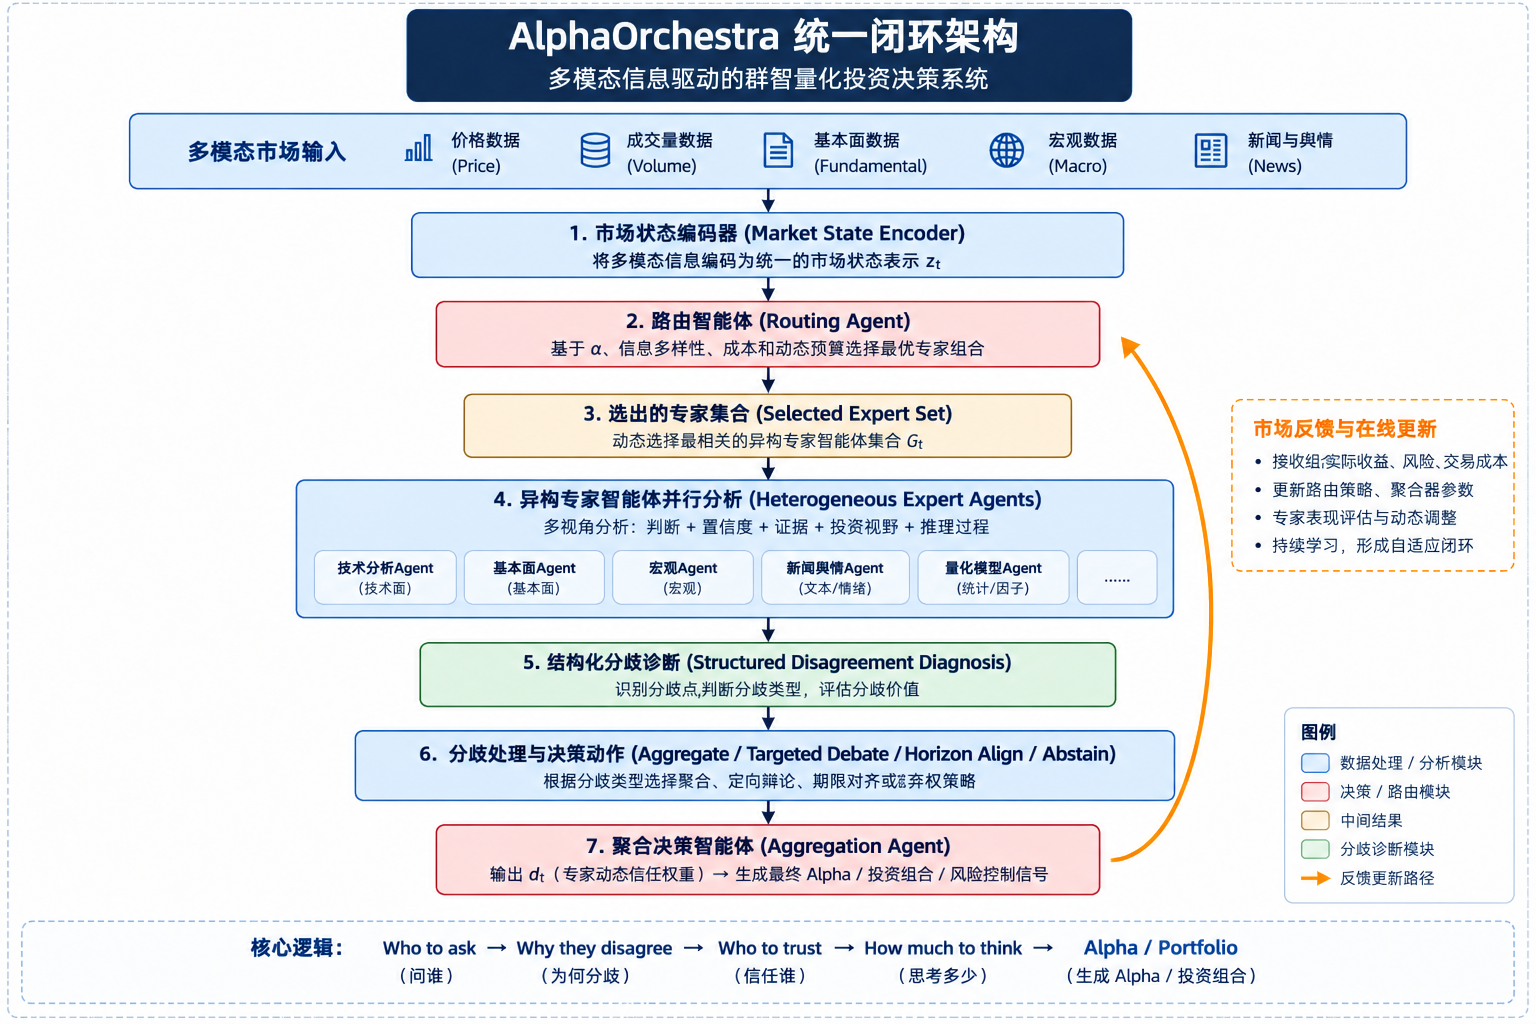
\includegraphics[width=0.96\linewidth]{media/image1.png}
\end{figure}

图1 AlphaOrchestra统一闭环：Selection → Expert Reasoning → Conflict
Resolution → Aggregation → Portfolio Feedback

\begin{figure}[H]
\centering
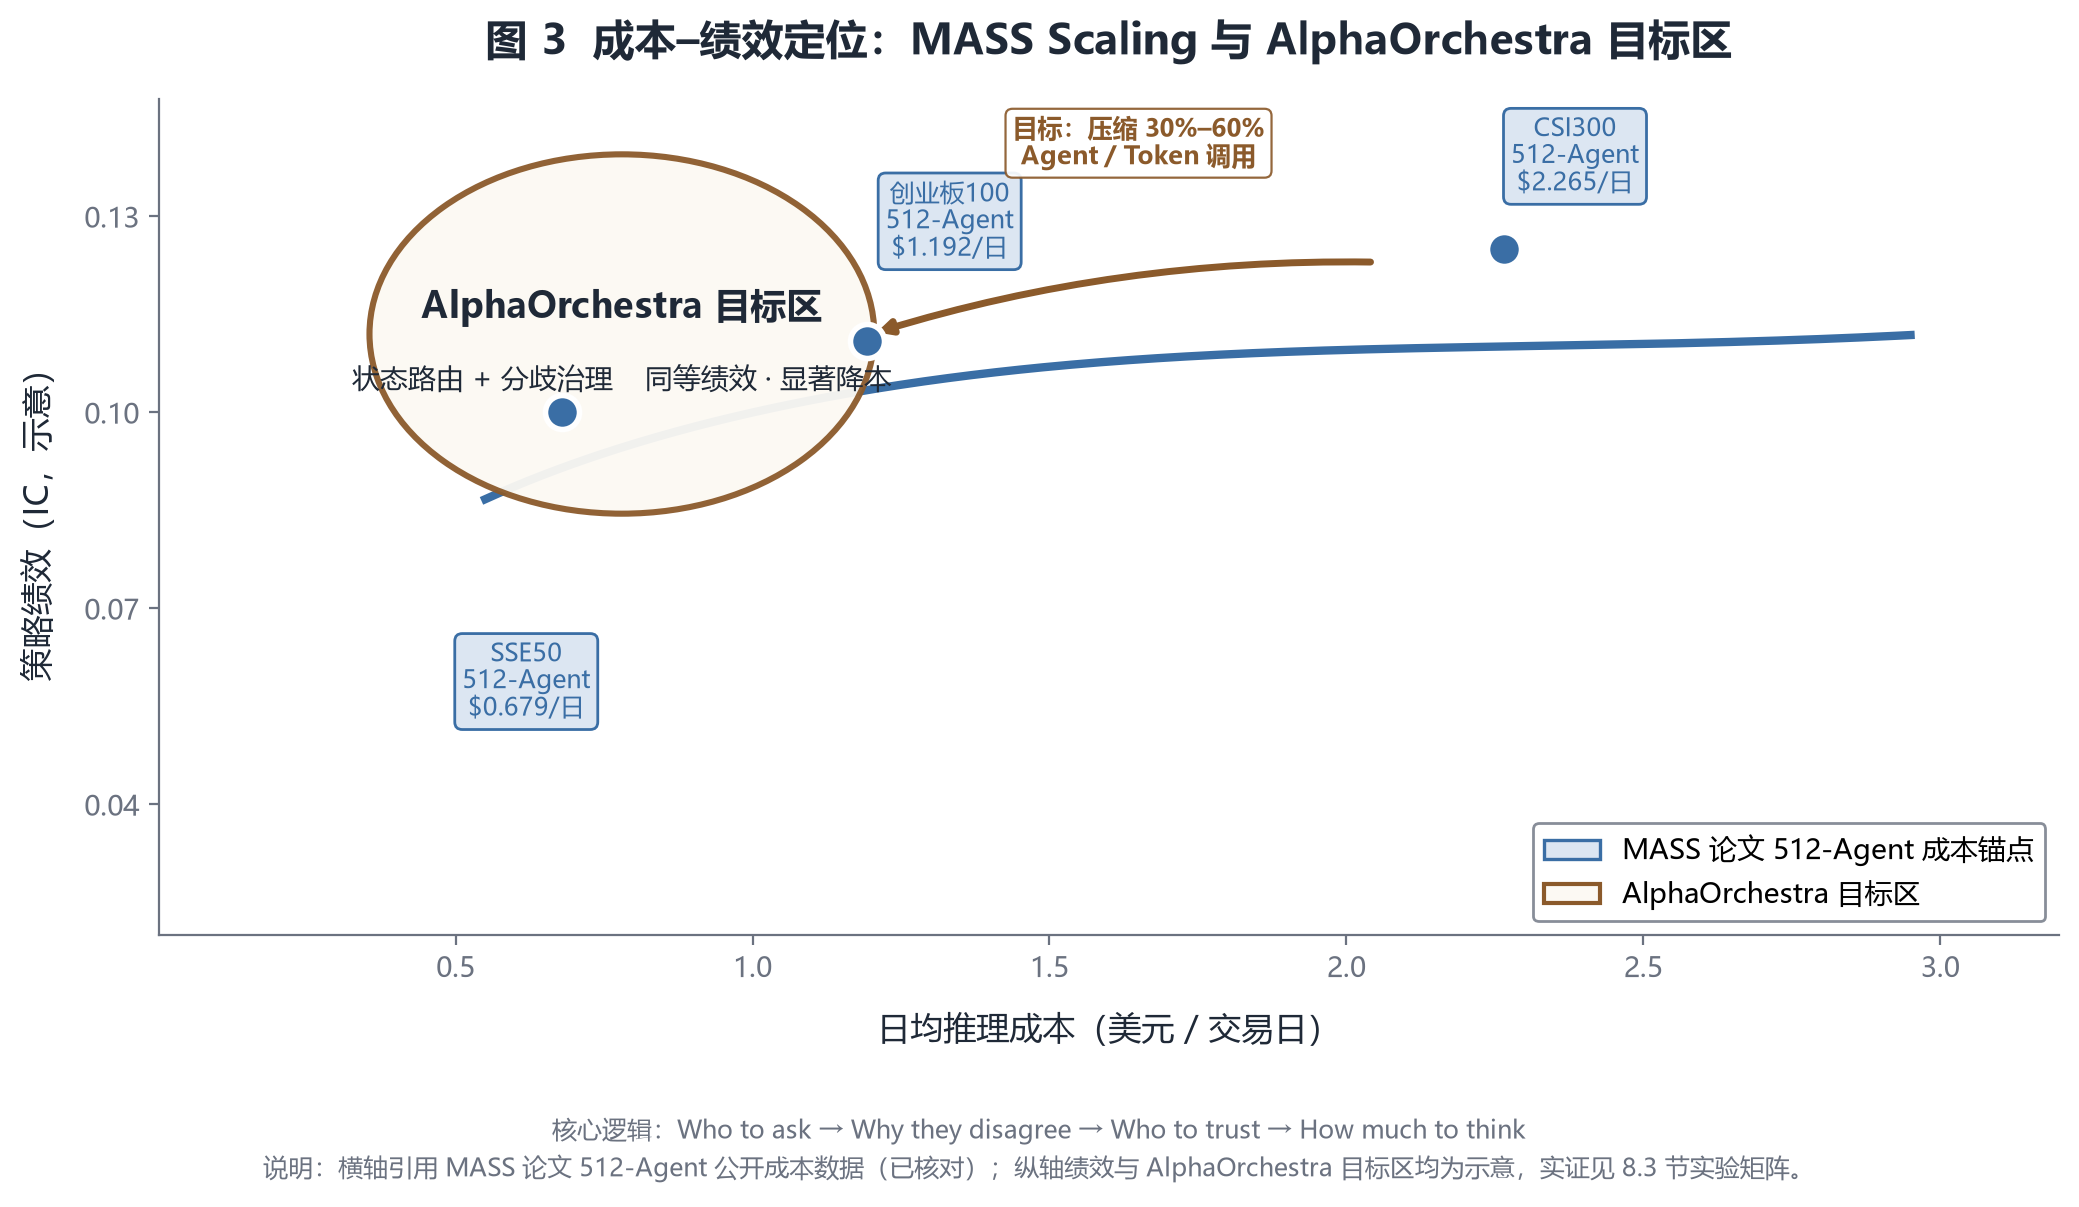
\includegraphics[width=0.96\linewidth]{media/image2.png}
\end{figure}

图3 成本--绩效定位：MASS Scaling（论文成本锚点）与 AlphaOrchestra
目标区（目标区为示意，实证见8.3节实验矩阵）

\subsection{\texorpdfstring{\textbf{5.1
Agent到底在哪里}}{5.1 Agent到底在哪里}}\label{agentux5230ux5e95ux5728ux54eaux91cc}

本项目中的``Agent''并不等于一个LLM
API调用。LLM可以承担Router/Diagnosis等控制器中的推理与解释能力，但完整Agent还包括状态、动作空间、工具、Memory、预算与停止规则。真正的智能体性体现在：同一个系统面对不同市场状态和不同冲突证据，会选择不同的专家集合、不同的Debate路径和不同的停止/弃权动作。

\subsection{\texorpdfstring{\textbf{5.2
每日运行流程}}{5.2 每日运行流程}}\label{ux6bcfux65e5ux8fd0ux884cux6d41ux7a0b}

\begin{enumerate}
\def\labelenumi{\arabic{enumi}.}
\item
  生成Market State
  Card：把价格、波动率、成交量、流动性、市场宽度、风格收益、宏观与文本事件编码为固定维向量zₜ={[}zₜ\^{}num,zₜ\^{}event{]}；zₜ\^{}num包括1/5/20日市场收益、20日实现波动率、成交额/换手、流动性、市场宽度、主要风格因子收益及利率、CPI、估值分位等宏观变量，并用滚动z-score或percentile标准化；zₜ\^{}event表示新闻、政策、财报等文本事件的类别特征或固定维embedding/projection。
\item
  Routing Agent读取zₜ、各Expert Type历史表现Hₜ、Profile
  P和预算Bₜ，输出Type-level调用变量gᵢ,ₜ∈\{0,1\}；其中i表示Expert/Investor
  Type，k表示该Type下的Individual Agent/replica。
\item
  仅被选中的Expert Type下的Individual
  Agents执行LLM/模型推理，并统一输出Prediction、Confidence、Horizon、Evidence、Reasoning；Type内多个replica可用于不同候选股票视图、随机采样或ensemble，并先聚合为该Type意见。
\item
  确定性程序计算结构化分歧特征；Diagnosis
  Agent解释主要冲突来源，并从Aggregate / Targeted Debate / Horizon Align
  / Abstain中选择动作。
\item
  Aggregation
  Agent综合市场状态、Type-level结构化输出、历史表现和历史权重先验d\_hist，输出Type-level动态信任权重dᵢ,ₜ，即问完以后信第i类专家多少。
\item
  形成Final Alpha
  Signal并交给Portfolio层；实盘/回测收益、风险、换手与推理成本回写Memory，更新Router、Aggregator与Expert
  Type/Individual Agent Reputation。
\end{enumerate}

\section{\texorpdfstring{\textbf{6.
三项核心创新}}{6. 三项核心创新}}\label{ux4e09ux9879ux6838ux5fc3ux521bux65b0}

\subsection{\texorpdfstring{\textbf{6.1 创新一：Dual-Stage Agent
Orchestration}}{6.1 创新一：Dual-Stage Agent Orchestration}}\label{ux521bux65b0ux4e00dual-stage-agent-orchestration}

\begin{longtable}[]{@{}
  >{\raggedright\arraybackslash}p{(\linewidth - 0\tabcolsep) * \real{1.0000}}@{}}
\toprule\noalign{}
\endhead
\bottomrule\noalign{}
\endlastfoot
\textbf{核心思想
先决定``问哪一类专家''（gᵢ,ₜ），再决定``信这一类专家多少''（dᵢ,ₜ）。这里i表示Expert/Investor
Type，k表示该Type下的Individual
Agent/replica；Type内输出先聚合为该Type意见。原MASS可理解为gᵢ,ₜ=1，即所有类型均参与，只动态学习dᵢ,ₜ；AlphaOrchestra在此基础上新增事前选择gᵢ,ₜ。} \\
\end{longtable}

Router输入由四部分组成：固定维市场状态zₜ；各Expert
Type近5/20日RankIC、hit
rate、回撤、不同Regime表现等历史能力Hₜ；数据模态、投资风格、预测期限、能力边界等Profile；以及当日Type数、Token/API费用、延迟等预算Bₜ。第一版可用Contextual
Gating Network（MLP + Top-K/阈值）产生调用价值qᵢ,ₜ，再得到gᵢ,ₜ∈\{0,1\}。

事后Aggregation不再只依赖近期收益，而是可表示为sᵢ,ₜ=fθ(zₜ,oᵢ,ₜ,Hᵢ,ₜ,dᵢ,ₜ\^{}hist)，再对被选Expert
Type做Softmax得到dᵢ,ₜ。这使系统能同时利用历史先验、当前市场状态和``该类专家今天具体说了什么''。

\textbf{当前实现状态：}Market State Encoder、Routing
Agent与信号聚合（Aggregation）的初版已实现，并已进入端到端验证实验闭环（见8.2节）。

\subsection{\texorpdfstring{\textbf{6.2 创新二：Structured Disagreement
Diagnosis}}{6.2 创新二：Structured Disagreement Diagnosis}}\label{ux521bux65b0ux4e8cstructured-disagreement-diagnosis}

\begin{longtable}[]{@{}
  >{\raggedright\arraybackslash}p{(\linewidth - 0\tabcolsep) * \real{1.0000}}@{}}
\toprule\noalign{}
\endhead
\bottomrule\noalign{}
\endlastfoot
\textbf{核心思想}
从``分歧有多大''升级为``为什么分歧，以及这种分歧应该被讨论、对齐、忽略还是用于降低风险''。 \\
\end{longtable}

代表性的共识---分歧聚合方法通常将分歧压缩为单一加权标准差σ。本项目要求Expert
Agent结构化输出，并以确定性程序计算分歧向量D={[}D\_pred,D\_evidence,D\_horizon,D\_conf,D\_semantic{]}：分别表示预测方向、证据集合、预测期限、置信度与语义推理差异。之后Diagnosis
Agent只能基于这些结构化证据给出冲突类别，例如model noise、information
conflict、horizon conflict、regime conflict、high uncertainty。

若 Fundamental Agent基于盈利改善看多而News/Policy
Agent基于监管事件看空，系统不会让所有Agent无限讨论，而是先统一投资期限，再向冲突双方提出同一个有边界的问题；若高分歧同时伴随普遍低置信度且Debate无法收敛，则输出系统置信度c\_sys并触发Abstain或降低仓位。这相当于给多智能体组合增加``我不知道''的能力。

冲突处理后的第i类专家对股票s在t时刻的预测记为p̃ᵢ,ₛ,ₜ：Aggregate保持原预测，Targeted
Debate使用讨论后的修正预测，Horizon
Align使用统一期限后的重新预测，Abstain通过系统置信度降低风险暴露而非强制生成方向。Aggregation
Agent输出dᵢ,ₜ=gᵢ,ₜexp(sᵢ,ₜ)/Σⱼgⱼ,ₜexp(sⱼ,ₜ)，其中sᵢ,ₜ为第i类专家trust
score，因此gᵢ,ₜ=0时dᵢ,ₜ=0且Σᵢdᵢ,ₜ=1。聚合预测μₛ,ₜ=Σᵢdᵢ,ₜp̃ᵢ,ₛ,ₜ，系统置信度c\_sysₛ,ₜ∈{[}0,1{]}，最终Alphaₛ,ₜ=c\_sysₛ,ₜμₛ,ₜ；当c\_sysₛ,ₜ\textless τ\_abstain时，可令该股票Alpha归零或显著降低对应风险暴露。

\textbf{当前实现状态：}分歧严重度计算与风险暴露控制（Exposure
Control）已实现并进入实验闭环；基于LLM的分歧归因解释与定向Debate机制已完成设计，为下一迭代重点。

\subsection{\texorpdfstring{\textbf{6.3 创新三：Diversity \& Cost-Aware
Adaptive
Computation}}{6.3 创新三：Diversity \& Cost-Aware Adaptive Computation}}\label{ux521bux65b0ux4e09diversity-cost-aware-adaptive-computation}

\begin{longtable}[]{@{}
  >{\raggedright\arraybackslash}p{(\linewidth - 0\tabcolsep) * \real{1.0000}}@{}}
\toprule\noalign{}
\endhead
\bottomrule\noalign{}
\endlastfoot
\textbf{核心思想 Raw Agent Count ≠ Effective Independent Information
Count。目标不是调用最多Agent，而是用最少的一组互补专家获得更高的有效信息密度。Innovation
1解决决策结构问题：在专家推理前新增独立Selection变量gₜ，并将其与事后Aggregation权重dₜ分离；Innovation
3解决Selection的优化目标问题：在既有Routing机制上进一步权衡信息价值、信息互补性和计算成本，并动态决定计算预算。} \\
\end{longtable}

系统为每个Expert Type维护长期Representation，包括Data
Modality、Investment Style、历史预测序列、Reasoning
Embedding、Token/Latency/API
Cost，并构造相似度Rᵢⱼ,ₜ。Router目标可写为：最大化 ΣᵢgᵢUᵢ,ₜ −
λΣᵢ\textless ⱼgᵢgⱼRᵢⱼ,ₜ −
ηΣᵢgᵢcᵢ,ₜ，即奖励预期信息/Alpha价值，惩罚专家冗余与推理成本。可计算定义为：Uᵢ,ₜ=w₁RankICᵢ,ₜ\^{}recent+w₂HitRateᵢ,ₜ+w₃RegimeScoreᵢ,ₜ，可用近5/20日滚动能力指标；Rᵢⱼ,ₜ=γ₁Corr(Predᵢ,Predⱼ)+γ₂CosSim(Reasonᵢ,Reasonⱼ)+γ₃DataOverlap(i,j)；cᵢ,ₜ=aTokenCostᵢ,ₜ+bLatencyᵢ,ₜ+cAPICostᵢ,ₜ。各项进入目标函数前统一尺度归一化。第一版用贪心选择即可，不必直接上复杂组合优化。

同时定义Market Complexity=f(Volatility, Event Intensity, OOD,
Uncertainty)，先形成事前Routing预算Bₜ\^{}route=f(MarketComplexityₜ)，在Expert
Agent执行前确定最大调用Expert Type数量与初始Token/API
Budget；收到专家输出并完成分歧诊断后，再形成事后Deliberation预算Bₛ,ₜ\^{}debate=f(MarketComplexityₜ,Dₛ,ₜ,Uncertaintyₛ,ₜ)，决定是否触发Debate、Debate轮数与额外Token
Budget。正常市场少问、少讨论；重大政策或极端波动时允许更多互补Agent和更高Debate预算。这样``How
much to think''是在推理过程中动态调整，也可以画出Performance--Cost
Frontier。（见图3）

\begin{longtable}[]{@{}
  >{\raggedright\arraybackslash}p{(\linewidth - 4\tabcolsep) * \real{0.2647}}
  >{\raggedright\arraybackslash}p{(\linewidth - 4\tabcolsep) * \real{0.4412}}
  >{\raggedright\arraybackslash}p{(\linewidth - 4\tabcolsep) * \real{0.2941}}@{}}
\toprule\noalign{}
\begin{minipage}[b]{\linewidth}\centering
\textbf{创新}
\end{minipage} & \begin{minipage}[b]{\linewidth}\centering
\textbf{最重要的消融问题}
\end{minipage} & \begin{minipage}[b]{\linewidth}\centering
\textbf{商业映射}
\end{minipage} \\
\midrule\noalign{}
\endhead
\bottomrule\noalign{}
\endlastfoot
双阶段编排 & 公开基线（MASS） vs Router-only vs Aggregator-only vs
Router+Aggregator & 减少无效调用、提升状态适应 \\
结构化分歧 & Consensus vs Consensus−σ vs Diagnosis vs
Diagnosis+Debate+Abstention & 降低``错误共识''和无意义争论 \\
多样性与成本 & Top-K vs Diversity-aware vs Diversity+Cost-aware &
直接形成Token/延迟/收益的ROI证据 \\
\end{longtable}

\textbf{当前实现状态：}路由模块已实现信息价值、信息差异与调用成本之间权衡的基础逻辑；完整的Agent相似度矩阵与动态计算预算为下一阶段规划工作。

\section{\texorpdfstring{\textbf{7.
工程实现与系统落地方案}}{7. 工程实现与系统落地方案}}\label{ux5de5ux7a0bux5b9eux73b0ux4e0eux7cfbux7edfux843dux5730ux65b9ux6848}

\subsection{\texorpdfstring{\textbf{7.1
为什么具备快速落地条件}}{7.1 为什么具备快速落地条件}}\label{ux4e3aux4ec0ux4e48ux5177ux5907ux5febux901fux843dux5730ux6761ux4ef6}

AlphaOrchestra采用独立、模块化的工程架构实现核心能力。公开论文、开源数据与公开实现主要用于相关工作研究、Benchmark复现和实验对照，以确保结果可比；项目核心的Market
State Encoder、Routing、Structured Disagreement、Diagnosis、Conditional
Debate、Adaptive Aggregation、Cost-aware Budget、Memory与Evidence
Trace由团队按照本项目架构自主设计与实现。

截至本版本，Market State
Encoder、Routing、基础分歧诊断与风险暴露控制的初版已由团队自主实现，并通过阶段性验证实验完成端到端流程检验（见8.2节）；定向Debate、Agent相似度矩阵与动态计算预算将在后续迭代中落地。

\subsection{\texorpdfstring{\textbf{7.2
核心模块实现位置}}{7.2 核心模块实现位置}}\label{ux6838ux5fc3ux6a21ux5757ux5b9eux73b0ux4f4dux7f6e}

\begin{longtable}[]{@{}
  >{\raggedright\arraybackslash}p{(\linewidth - 4\tabcolsep) * \real{0.2571}}
  >{\raggedright\arraybackslash}p{(\linewidth - 4\tabcolsep) * \real{0.3029}}
  >{\raggedright\arraybackslash}p{(\linewidth - 4\tabcolsep) * \real{0.4400}}@{}}
\toprule\noalign{}
\begin{minipage}[b]{\linewidth}\centering
\textbf{AlphaOrchestra核心模块}
\end{minipage} & \begin{minipage}[b]{\linewidth}\centering
\textbf{主要职责}
\end{minipage} & \begin{minipage}[b]{\linewidth}\centering
\textbf{自主实现重点}
\end{minipage} \\
\midrule\noalign{}
\endhead
\bottomrule\noalign{}
\endlastfoot
orchestration/executor.py & 交易日级任务编排与Agent执行 &
在执行前接入Market State + Router，仅提交selected
agents；记录调用成本与路由轨迹 \\
routing/router.py & 基于zₜ、Hₜ、Profile、Budget输出gₜ & 实现Type-level
selection，并记录路由分数与未选择原因 \\
agents/expert\_agent.py + prompts & 异构LLM专家生成策略与股票判断 &
统一JSON Schema：prediction/confidence/horizon/evidence/reasoning \\
aggregation/signal\_engine.py & 计算基础共识/分歧并形成候选信号 &
加入structured disagreement、diagnosis动作与adaptive aggregation \\
diagnosis/disagreement.py &
计算D\_pred、D\_evidence、D\_horizon、D\_conf、D\_semantic并提供Diagnosis接口
& 保持确定性分歧特征与LLM归因解释解耦 \\
optimization/reputation.py & 维护历史Agent能力、信誉与动态权重先验 &
使用d\_hist作为历史先验，并与Aggregator/Router学习权重及成本目标联动 \\
memory/agent\_registry.py & 维护Agent长期状态与决策记忆 & 保存Agent
Profile、相似度、历史Regime表现、Debate记录、Token/latency、reputation \\
risk/optimizer\_adapter.py & 连接风险模型与组合优化器 &
商业版以接口方式接入机构现有风险模型/组合优化器，Agent不绕过硬约束 \\
cost/budget\_manager.py & 跟踪Token/API/Latency并管理ex-ante / ex-post
budget & 支持Routing预算与Deliberation预算分阶段控制 \\
\end{longtable}

\subsection{\texorpdfstring{\textbf{7.3
LLM与确定性计算的边界}}{7.3 LLM与确定性计算的边界}}\label{llmux4e0eux786eux5b9aux6027ux8ba1ux7b97ux7684ux8fb9ux754c}

\begin{longtable}[]{@{}
  >{\raggedright\arraybackslash}p{(\linewidth - 4\tabcolsep) * \real{0.2941}}
  >{\raggedright\arraybackslash}p{(\linewidth - 4\tabcolsep) * \real{0.2941}}
  >{\raggedright\arraybackslash}p{(\linewidth - 4\tabcolsep) * \real{0.4118}}@{}}
\toprule\noalign{}
\begin{minipage}[b]{\linewidth}\centering
\textbf{任务}
\end{minipage} & \begin{minipage}[b]{\linewidth}\centering
\textbf{执行主体}
\end{minipage} & \begin{minipage}[b]{\linewidth}\centering
\textbf{原因}
\end{minipage} \\
\midrule\noalign{}
\endhead
\bottomrule\noalign{}
\endlastfoot
IC/RankIC、收益、风险、相似度、Token计费 & Python/统计程序 &
必须确定、可复现 \\
Market numeric state & 数值模型/规则 &
避免LLM``凭感觉''判断波动和流动性 \\
冲突解释、定向问题生成 & LLM Diagnosis/Critic &
需要语义理解与跨模态理由整合 \\
Router第一版 & MLP/规则 + 可选LLM解释 &
选择本身要可验证，LLM解释不能替代数值Score \\
Portfolio hard constraints & 传统Optimizer/风控系统 &
行业、Beta、单票、换手等硬约束不可由LLM覆盖 \\
\end{longtable}

\section{\texorpdfstring{\textbf{8.
数据、实验与评价体系}}{8. 数据、实验与评价体系}}\label{ux6570ux636eux5b9eux9a8cux4e0eux8bc4ux4ef7ux4f53ux7cfb}

\subsection{\texorpdfstring{\textbf{8.1
数据与基线}}{8.1 数据与基线}}\label{ux6570ux636eux4e0eux57faux7ebf}

公开研究中的A股多智能体数据设置覆盖SSE50、CSI300、创业板100等股票池，包含新闻、财报摘要、价量、基本面及宏观指标；公开资源中也提供了可用于复现实验的SSE50示例数据。第一阶段优先在公开SSE50数据上建立统一Benchmark，随后如具备数据权限，再扩展CSI300/CSI
A500或比赛指定数据。正式实验中的公开基线MASS将区分MASS-Paper（按论文公式与参数实现）与MASS-Code（按官方开源仓库当前实现运行），以避免论文描述与公开实现口径差异影响公平比较。所有新增数据必须遵守Point-in-Time可得性，训练、路由、聚合和回测均不得使用未来信息。

\subsection{\texorpdfstring{\textbf{8.2
阶段性验证实验（已完成）}}{8.2 阶段性验证实验（已完成）}}\label{ux9636ux6bb5ux6027ux9a8cux8bc1ux5b9eux9a8cux5df2ux5b8cux6210}

在进入大规模消融实验之前，团队已在公开SSE50示例数据上完成系统端到端验证实验。实验设置为：两类投资者类型智能体（num\_investor\_type=2，每类1个Agent），候选股票池10只、每日选择3只，时间区间2023年1月3日至2023年1月31日，共16个交易日。系统完整执行了从数据读取、智能体初始化、市场状态编码、智能体路由、投资判断、分歧诊断、信号聚合到IC评估的全流程，LLM服务通过环境变量配置并完成DeepSeek等OpenAI格式接口适配。各预测周期的IC评估结果如下：

\begin{longtable}[]{@{}
  >{\raggedright\arraybackslash}p{(\linewidth - 8\tabcolsep) * \real{0.2000}}
  >{\centering\arraybackslash}p{(\linewidth - 8\tabcolsep) * \real{0.2000}}
  >{\centering\arraybackslash}p{(\linewidth - 8\tabcolsep) * \real{0.2000}}
  >{\centering\arraybackslash}p{(\linewidth - 8\tabcolsep) * \real{0.2000}}
  >{\centering\arraybackslash}p{(\linewidth - 8\tabcolsep) * \real{0.2000}}@{}}
\toprule\noalign{}
\endhead
\bottomrule\noalign{}
\endlastfoot
\textbf{预测周期} & \textbf{IC} & \textbf{ICIR} & \textbf{RankIC} &
\textbf{RankICIR} \\
1日 & 0.0026 & 0.0342 & 0.0247 & 0.2413 \\
5日 & -0.0762 & -0.6935 & -0.0916 & -0.6742 \\
10日 & -0.0666 & -1.9825 & -0.0742 & -1.4008 \\
\end{longtable}

从结果看，1日预测周期的IC与RankIC在该小样本测试中为正，但样本仅包含16个交易日，当前结果不足以支持统计显著的预测能力结论；5日与10日周期结果偏弱，符合系统完成主流程搭建初期的预期------智能体数量、样本长度、聚合参数与提示词鲁棒性尚未充分优化。当前阶段性实验尚未对Consensus与不同类型Disagreement的独立预测信息进行充分分解，该问题将在8.3节Innovation
2的正式消融实验中通过Consensus、Consensus−σ、Diagnosis及Diagnosis+Debate+Abstain的统一对比进行验证。

需要明确的是，本轮实验的主要目的在于验证从数据读取、市场状态编码、Agent路由、投资判断、分歧处理、信号聚合到评价指标计算的端到端工程闭环能够稳定运行，而非得出最终策略绩效结论；更严格的结论将在第8.3节核心实验矩阵的大规模消融、性能--成本前沿与Regime解释性实验中得出。

\subsection{\texorpdfstring{\textbf{8.3
核心实验矩阵}}{8.3 核心实验矩阵}}\label{ux6838ux5fc3ux5b9eux9a8cux77e9ux9635}

\begin{longtable}[]{@{}
  >{\raggedright\arraybackslash}p{(\linewidth - 4\tabcolsep) * \real{0.1941}}
  >{\raggedright\arraybackslash}p{(\linewidth - 4\tabcolsep) * \real{0.4235}}
  >{\raggedright\arraybackslash}p{(\linewidth - 4\tabcolsep) * \real{0.3823}}@{}}
\toprule\noalign{}
\begin{minipage}[b]{\linewidth}\centering
\textbf{实验}
\end{minipage} & \begin{minipage}[b]{\linewidth}\centering
\textbf{对比组}
\end{minipage} & \begin{minipage}[b]{\linewidth}\centering
\textbf{主要回答的问题}
\end{minipage} \\
\midrule\noalign{}
\endhead
\bottomrule\noalign{}
\endlastfoot
Innovation 1 & 公开基线MASS（MASS-Paper / MASS-Code） / Router-only /
Aggregator-only / Router+Aggregator & 事前选择与事后信任是否都有增益 \\
Innovation 2 & Consensus / Consensus−σ / Diagnosis /
Diagnosis+Debate+Abstain & 结构化冲突处理是否优于统一惩罚 \\
Innovation 3 & Top-K / Diversity-aware / Diversity+Cost-aware &
互补性是否提升有效信息；相同表现下能否减少调用成本 \\
Full System & 公开强基线（含MASS-Paper / MASS-Code） vs AlphaOrchestra &
综合收益、风险、换手、成本与解释性是否改善 \\
Stress/OOS & 不同Regime、不同股票池、不同LLM、不同预算 &
效果是否依赖单一模型或单一市场环境 \\
\end{longtable}

\subsection{\texorpdfstring{\textbf{8.4
评价指标}}{8.4 评价指标}}\label{ux8bc4ux4ef7ux6307ux6807}

\begin{longtable}[]{@{}
  >{\raggedright\arraybackslash}p{(\linewidth - 2\tabcolsep) * \real{0.2353}}
  >{\raggedright\arraybackslash}p{(\linewidth - 2\tabcolsep) * \real{0.7647}}@{}}
\toprule\noalign{}
\begin{minipage}[b]{\linewidth}\centering
\textbf{维度}
\end{minipage} & \begin{minipage}[b]{\linewidth}\centering
\textbf{指标}
\end{minipage} \\
\midrule\noalign{}
\endhead
\bottomrule\noalign{}
\endlastfoot
预测质量 & RankIC、IC、RICIR/ICIR、Hit Rate \\
组合绩效 & Annualized Return、Sharpe、Max Drawdown、Excess Return \\
交易可行性 & Turnover、Transaction Cost、持仓集中度 \\
Agent效率 & Agent Calls、Token/API Cost、Latency、Performance--Cost
Frontier \\
自适应性 & Regime切换恢复时间、不同Regime下Selection分布 \\
冲突治理 & Debate Trigger Rate、Resolution Success、Abstention Rate \\
可解释性 & Selection理由可追溯率、Evidence Coverage、决策轨迹复现率 \\
\end{longtable}

\subsection{\texorpdfstring{\textbf{8.5
数据泄漏与统计可信度}}{8.5 数据泄漏与统计可信度}}\label{ux6570ux636eux6cc4ux6f0fux4e0eux7edfux8ba1ux53efux4fe1ux5ea6}

现有多智能体金融研究已经专门讨论LLM历史记忆导致的数据泄漏风险，并通过未见数据进行额外验证。本项目进一步要求所有Router/Aggregator学习只使用决策时点以前的市场信息；任何用未来收益计算出的能力分数只能在其真实可获得后进入下一期Memory。最终报告应同时展示Walk-forward/OOS、不同seed，以及在可能条件下的跨股票池验证，避免把单次回测最优当作产品能力。

\section{\texorpdfstring{\textbf{9.
MVP、演示与产品形态}}{9. MVP、演示与产品形态}}\label{mvpux6f14ux793aux4e0eux4ea7ux54c1ux5f62ux6001}

\begin{figure}[H]
\centering
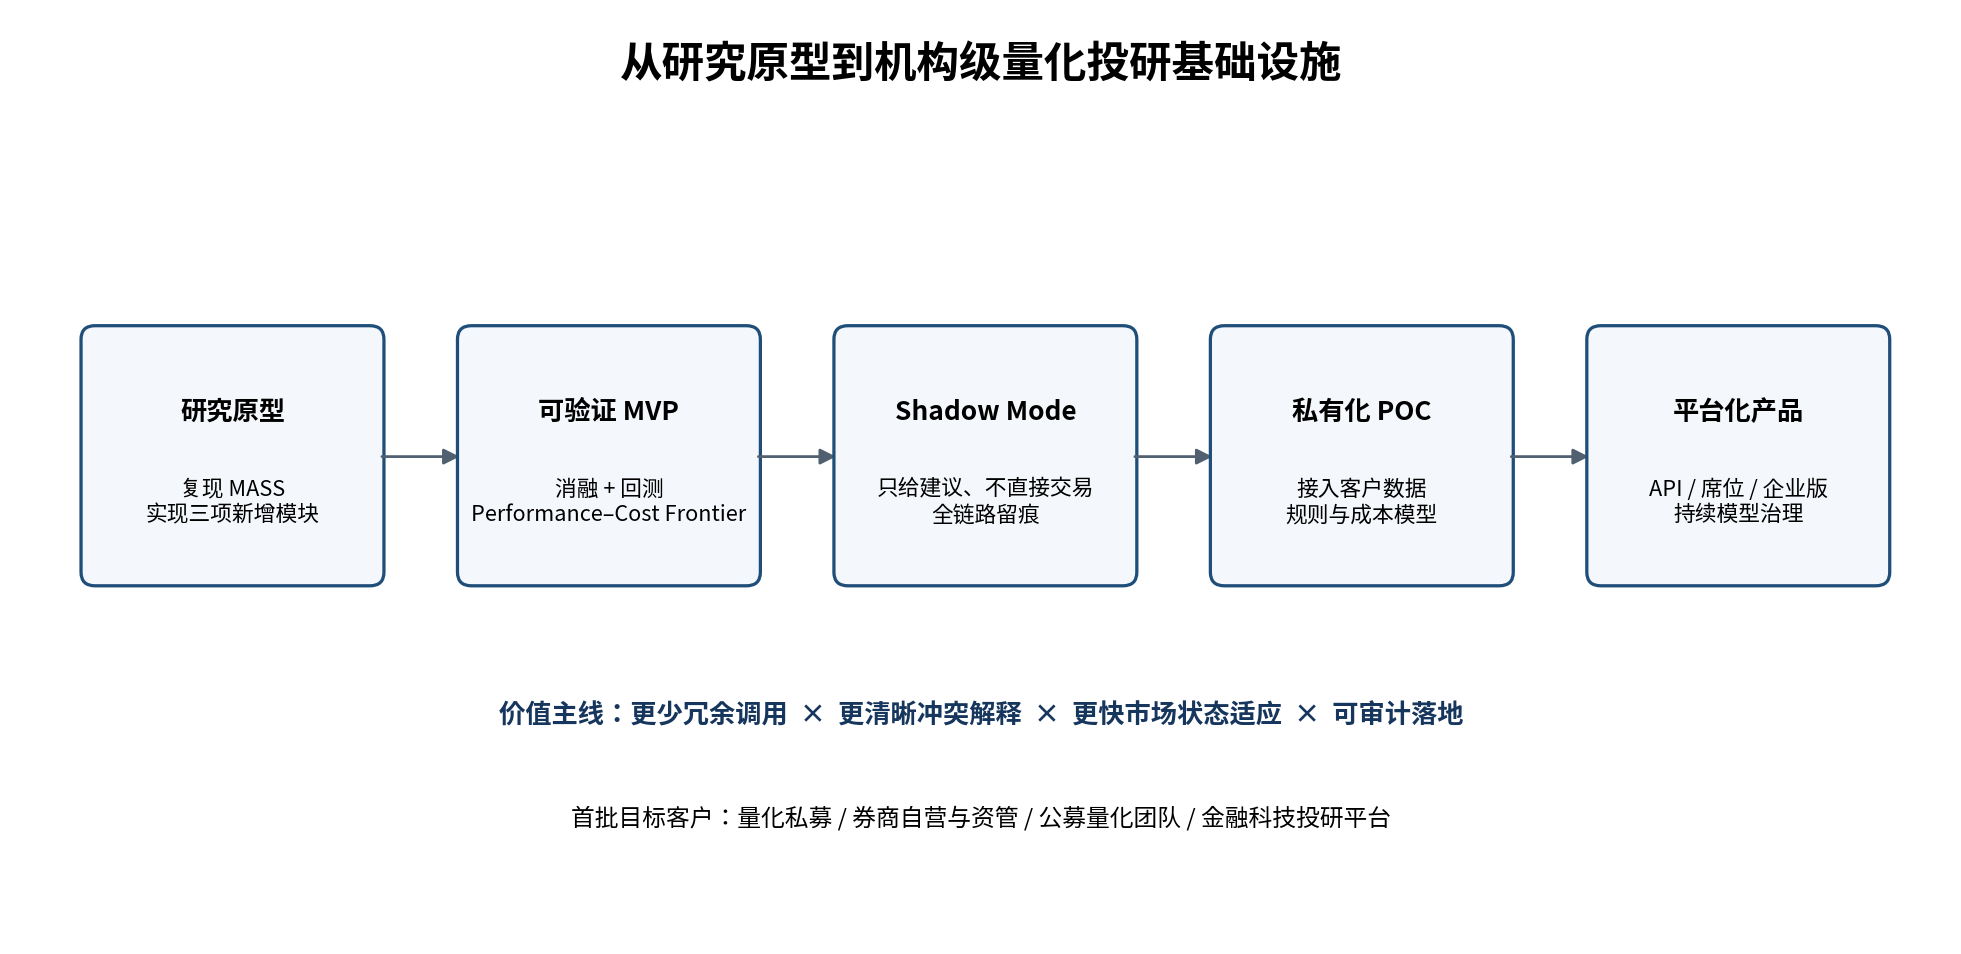
\includegraphics[width=0.96\linewidth]{media/image3.png}
\end{figure}

图2 商业化路径：从可复现实验到Shadow Mode再到私有化部署

\subsection{\texorpdfstring{\textbf{9.1
MVP核心演示场景：可观测的多智能体动态决策闭环}}{9.1 MVP核心演示场景：可观测的多智能体动态决策闭环}}\label{mvpux6838ux5fc3ux6f14ux793aux573aux666fux53efux89c2ux6d4bux7684ux591aux667aux80fdux4f53ux52a8ux6001ux51b3ux7b56ux95edux73af}

MVP选取具有显著市场状态变化的典型交易日或时间窗口，展示 AlphaOrchestra
从市场状态识别、专家路由、分歧诊断到动态聚合的端到端决策过程。当前已完成的阶段性Demo包括Market
State Encoder、基础Routing、Expert执行、基础disagreement severity /
exposure control、Signal Aggregation、IC /
RankIC评价与基础调用Trace。系统首先生成Market State Card；Routing
Agent根据当前市场状态、专家历史表现与预算，从候选Expert
Type池中选择一组异构专家，而非固定调用全部Agent。各专家按照统一结构输出预测方向、置信度、证据、投资期限与推理依据；现阶段已支持基础分歧严重度识别与风险暴露控制，比赛最终MVP计划补齐LLM-based
disagreement attribution、Targeted Debate、Agent Similarity
Matrix、Dynamic Computation Budget与更完整Conflict
Console。最终，Aggregation
Agent根据市场状态、历史先验与经冲突处理后的Type-level专家意见生成动态信任权重dₜ，形成最终Alpha排序与组合决策信号。系统同时记录Agent调用数量、Token消耗、推理时延等运行指标，用于量化比较全量调用与自适应编排机制在投资表现与计算成本之间的效率差异。

\subsection{\texorpdfstring{\textbf{9.2
MVP四个页面}}{9.2 MVP四个页面}}\label{mvpux56dbux4e2aux9875ux9762}

\begin{longtable}[]{@{}
  >{\raggedright\arraybackslash}p{(\linewidth - 4\tabcolsep) * \real{0.2118}}
  >{\raggedright\arraybackslash}p{(\linewidth - 4\tabcolsep) * \real{0.4118}}
  >{\raggedright\arraybackslash}p{(\linewidth - 4\tabcolsep) * \real{0.3764}}@{}}
\toprule\noalign{}
\begin{minipage}[b]{\linewidth}\centering
\textbf{页面}
\end{minipage} & \begin{minipage}[b]{\linewidth}\centering
\textbf{内容}
\end{minipage} & \begin{minipage}[b]{\linewidth}\centering
\textbf{评委看到的价值}
\end{minipage} \\
\midrule\noalign{}
\endhead
\bottomrule\noalign{}
\endlastfoot
Market \& Agent Map & Regime、Agent Profile、历史表现、相似度 &
系统知道``现在是什么市场''和``每个专家擅长什么'' \\
Routing Trace & 谁被选/没被选、Selection Score、成本 &
动态组队，不是固定流水线 \\
Conflict Console & 预测、证据、期限、置信度、冲突类型、Debate &
分歧被解释和处理，而非统一扣分 \\
Portfolio \& Cost & 最终Alpha、权重、收益风险、Token/延迟、基线对比 &
同时证明效果与工程经济性 \\
\end{longtable}

注：当前实验链路已支持上述四页中已实现模块的数据产出；完整四页MVP将在补齐Targeted
Debate、Agent Similarity Matrix与Dynamic Budget后形成。

\subsection{\texorpdfstring{\textbf{9.3
POC版产品形态}}{9.3 POC版产品形态}}\label{pocux7248ux4ea7ux54c1ux5f62ux6001}

机构POC建议采用私有化或VPC部署，数据不出域。Agent编排层以API连接客户已有行情、因子库、LLM
Gateway、风险模型与回测器；部署前先运行4--8周Shadow
Mode，仅输出建议与完整Trace，不直接影响真实仓位。达到预设稳定性、成本和风险门槛后，再由客户决定是否进入人机协同流程。

\section{\texorpdfstring{\textbf{10.
目标市场与客户画像}}{10. 目标市场与客户画像}}\label{ux76eeux6807ux5e02ux573aux4e0eux5ba2ux6237ux753bux50cf}

\subsection{\texorpdfstring{\textbf{10.1
市场不是``全中国AUM''，而是可付费的机构投研软件预算}}{10.1 市场不是``全中国AUM''，而是可付费的机构投研软件预算}}\label{ux5e02ux573aux4e0dux662fux5168ux4e2dux56fdaumux800cux662fux53efux4ed8ux8d39ux7684ux673aux6784ux6295ux7814ux8f6fux4ef6ux9884ux7b97}

市场测算采用自下而上方法，不把7万亿元私募证券基金规模直接当作软件TAM。初始客户单元是``拥有系统化投研团队、可提供结构化数据、具有LLM/AI试点预算、且对私有化和合规有明确要求的机构''。

\begin{longtable}[]{@{}
  >{\raggedright\arraybackslash}p{(\linewidth - 4\tabcolsep) * \real{0.2353}}
  >{\raggedright\arraybackslash}p{(\linewidth - 4\tabcolsep) * \real{0.4705}}
  >{\raggedright\arraybackslash}p{(\linewidth - 4\tabcolsep) * \real{0.2941}}@{}}
\toprule\noalign{}
\begin{minipage}[b]{\linewidth}\centering
\textbf{市场层级}
\end{minipage} & \begin{minipage}[b]{\linewidth}\centering
\textbf{口径（规划假设）}
\end{minipage} & \begin{minipage}[b]{\linewidth}\centering
\textbf{年收入机会测算}
\end{minipage} \\
\midrule\noalign{}
\endhead
\bottomrule\noalign{}
\endlastfoot
Beachhead / SOM & 三年内15家付费机构，平均年合同60万元 & 约900万元/年 \\
初始SAM & 约300家量化/系统化程度较高机构 × 50万元年客单 &
约1.5亿元/年 \\
扩展SAM & 约800家私募、券商资管、公募/金融科技机构 × 50万元 &
约4亿元/年 \\
\end{longtable}

上述机构数量与客单价均是商业规划假设，用于展示单位经济模型，而不是外部审计的行业市场规模。正式融资或商业化前应通过20--30家目标客户访谈校正。

\subsection{\texorpdfstring{\textbf{10.2
客户画像与购买触发点}}{10.2 客户画像与购买触发点}}\label{ux5ba2ux6237ux753bux50cfux4e0eux8d2dux4e70ux89e6ux53d1ux70b9}

\begin{longtable}[]{@{}
  >{\raggedright\arraybackslash}p{(\linewidth - 6\tabcolsep) * \real{0.2177}}
  >{\raggedright\arraybackslash}p{(\linewidth - 6\tabcolsep) * \real{0.3411}}
  >{\raggedright\arraybackslash}p{(\linewidth - 6\tabcolsep) * \real{0.2059}}
  >{\raggedright\arraybackslash}p{(\linewidth - 6\tabcolsep) * \real{0.2353}}@{}}
\toprule\noalign{}
\begin{minipage}[b]{\linewidth}\centering
\textbf{客户}
\end{minipage} & \begin{minipage}[b]{\linewidth}\centering
\textbf{典型触发点}
\end{minipage} & \begin{minipage}[b]{\linewidth}\centering
\textbf{主要采购人}
\end{minipage} & \begin{minipage}[b]{\linewidth}\centering
\textbf{价值证明}
\end{minipage} \\
\midrule\noalign{}
\endhead
\bottomrule\noalign{}
\endlastfoot
百亿/中大型量化私募 & Agent调用成本高、策略拥挤、需要多模态研究 &
投研负责人/CTO & 同表现降成本、Regime适应、Trace \\
券商自营/资管 & 合规与系统治理要求更高 & 量化负责人/科技/风险 &
私有化、权限、审计、硬风险约束 \\
公募量化/指数增强 & 需要稳定性与研究协同 & 基金经理/量化研究 &
稳健性、组合风险、研究可复现 \\
金融科技平台 & 希望增强现有回测/因子平台Agent能力 & 产品/算法负责人 &
可插拔Agentic Control Plane \\
\end{longtable}

\section{\texorpdfstring{\textbf{11.
竞争格局与差异化壁垒}}{11. 竞争格局与差异化壁垒}}\label{ux7adeux4e89ux683cux5c40ux4e0eux5deeux5f02ux5316ux58c1ux5792}

\subsection{\texorpdfstring{\textbf{11.1
竞争不是``没有竞品''，而是四类替代方案}}{11.1 竞争不是``没有竞品''，而是四类替代方案}}\label{ux7adeux4e89ux4e0dux662fux6ca1ux6709ux7adeux54c1ux800cux662fux56dbux7c7bux66ffux4ee3ux65b9ux6848}

\begin{longtable}[]{@{}
  >{\raggedright\arraybackslash}p{(\linewidth - 6\tabcolsep) * \real{0.2105}}
  >{\raggedright\arraybackslash}p{(\linewidth - 6\tabcolsep) * \real{0.2515}}
  >{\raggedright\arraybackslash}p{(\linewidth - 6\tabcolsep) * \real{0.2456}}
  >{\raggedright\arraybackslash}p{(\linewidth - 6\tabcolsep) * \real{0.2924}}@{}}
\toprule\noalign{}
\begin{minipage}[b]{\linewidth}\centering
\textbf{类别}
\end{minipage} & \begin{minipage}[b]{\linewidth}\centering
\textbf{代表/现状}
\end{minipage} & \begin{minipage}[b]{\linewidth}\centering
\textbf{优势}
\end{minipage} & \begin{minipage}[b]{\linewidth}\centering
\textbf{AlphaOrchestra差异}
\end{minipage} \\
\midrule\noalign{}
\endhead
\bottomrule\noalign{}
\endlastfoot
传统量化平台 & Qlib、自研回测/因子平台 & 可靠、成熟、工具丰富 &
在其上增加多Agent选择、冲突治理和成本编排，不替换底层工具 \\
单/多Agent交易框架 & TradingAgents、FinCON等 & 角色分工、自然语言推理 &
更聚焦事前动态路由、结构化分歧和成本--多样性目标 \\
多Agent组合研究 & MASS等 & 大规模异构Agent与动态权重提供了重要研究参照 &
AlphaOrchestra进一步强调事前动态组队、结构化冲突治理与动态计算预算 \\
机构内部人工流程 & 研究员手工看多个模型/报告 & 经验强、可灵活判断 &
把重复的``找专家---对冲突---做记录''结构化、自动化和可复现 \\
\end{longtable}

Qlib本身覆盖数据处理、模型训练、回测、风险、组合优化和执行等完整量化链路，并已引入RD-Agent做自动R\&D。AlphaOrchestra不应宣称替代Qlib，而应将其视为可连接的Quant
Tool
Layer；真正差异化的是``跨异构投资Agent的动态选择---冲突诊断---成本治理''。

对最重要的公开参照MASS，竞合边界可以一句话界定：MASS验证了``Agent越多越强''的规模化方向；AlphaOrchestra在此基础上解决规模化之后的经济性与治理问题------同等绩效下压缩Agent/Token调用、让冲突可审计可干预。MASS论文与开源代码将作为本项目消融实验的公开基线，核验结果以可复现方式回馈开源社区。

\subsection{\texorpdfstring{\textbf{11.2
可形成的五类壁垒}}{11.2 可形成的五类壁垒}}\label{ux53efux5f62ux6210ux7684ux4e94ux7c7bux58c1ux5792}

\begin{longtable}[]{@{}
  >{\raggedright\arraybackslash}p{(\linewidth - 2\tabcolsep) * \real{0.2470}}
  >{\raggedright\arraybackslash}p{(\linewidth - 2\tabcolsep) * \real{0.7530}}@{}}
\toprule\noalign{}
\begin{minipage}[b]{\linewidth}\centering
\textbf{壁垒}
\end{minipage} & \begin{minipage}[b]{\linewidth}\centering
\textbf{形成方式}
\end{minipage} \\
\midrule\noalign{}
\endhead
\bottomrule\noalign{}
\endlastfoot
数据壁垒 &
客户私有数据上的Regime---Agent能力矩阵与冲突历史，不需要外泄原始数据 \\
经验壁垒 & Agent Reputation、相似度与Debate outcome构成可持续Memory \\
系统壁垒 & Router、Diagnosis、Aggregator与量化Tool
API形成完整可治理控制面 \\
评估壁垒 & Performance--Cost
Frontier、Regime恢复、冲突解决等专有评测体系 \\
交付壁垒 &
金融机构私有化、权限、审计、Fallback与Human-in-the-loop工程经验 \\
\end{longtable}

\section{\texorpdfstring{\textbf{12.
商业模式与定价}}{12. 商业模式与定价}}\label{ux5546ux4e1aux6a21ux5f0fux4e0eux5b9aux4ef7}

\subsection{\texorpdfstring{\textbf{12.1
商业模式}}{12.1 商业模式}}\label{ux5546ux4e1aux6a21ux5f0f}

项目采取B2B``POC → 私有化订阅/License →
企业级平台/API''的渐进模式。早期不以公开SaaS直接处理客户核心交易数据，而以私有化部署和Shadow
Mode降低信任门槛。收入由软件许可、部署与适配服务、增值模块和可选推理资源管理组成。

\begin{longtable}[]{@{}
  >{\raggedright\arraybackslash}p{(\linewidth - 4\tabcolsep) * \real{0.2353}}
  >{\raggedright\arraybackslash}p{(\linewidth - 4\tabcolsep) * \real{0.2765}}
  >{\raggedright\arraybackslash}p{(\linewidth - 4\tabcolsep) * \real{0.4882}}@{}}
\toprule\noalign{}
\begin{minipage}[b]{\linewidth}\centering
\textbf{产品层级}
\end{minipage} & \begin{minipage}[b]{\linewidth}\centering
\textbf{建议价格（规划值）}
\end{minipage} & \begin{minipage}[b]{\linewidth}\centering
\textbf{交付内容}
\end{minipage} \\
\midrule\noalign{}
\endhead
\bottomrule\noalign{}
\endlastfoot
研究POC & 8--20万元 / 4--8周 &
1个股票池、1--2个LLM、Router/Diagnosis/Aggregator、对比实验与报告 \\
Research Edition & 30--80万元/年 &
私有部署、多个策略/股票池、用户权限、Trace、成本看板、年度升级 \\
Enterprise Edition & 80--200万元/年起 &
高可用、模型网关、风控/回测系统集成、审计、SLA、定制Agent Registry \\
API / Academic & 按席位或调用量 &
适合平台方、科研机构或非敏感数据场景 \\
\end{longtable}

价格为参赛阶段的建议报价区间，尚未经过真实客户成交验证。提交前最好完成至少5--10次目标客户访谈，把``愿意付多少钱''与``采购流程多久''写成访谈证据。

\subsection{\texorpdfstring{\textbf{12.2
客户ROI的计算方式}}{12.2 客户ROI的计算方式}}\label{ux5ba2ux6237roiux7684ux8ba1ux7b97ux65b9ux5f0f}

不把ROI写成``增加多少收益''单一维度，而用三条可审计公式：①推理节省 =
基线Agent Calls/Token − 实际Calls/Token；②研究效率 =
单个可接受策略/信号所需的实验轮次与工程小时；③风险收益 =
相同或更低MDD/Turnover条件下的RankIC/Sharpe变化。对于客户而言，只要系统能在接近投资表现的前提下显著降低大模型调用、研究重复与治理成本，就有独立于``收益承诺''的付费理由。

\section{\texorpdfstring{\textbf{13.
市场进入与机构落地路径}}{13. 市场进入与机构落地路径}}\label{ux5e02ux573aux8fdbux5165ux4e0eux673aux6784ux843dux5730ux8defux5f84}

\subsection{\texorpdfstring{\textbf{13.1
先从``研究工具''切入，而不是直接申请交易权限}}{13.1 先从``研究工具''切入，而不是直接申请交易权限}}\label{ux5148ux4eceux7814ux7a76ux5de5ux5177ux5207ux5165ux800cux4e0dux662fux76f4ux63a5ux7533ux8bf7ux4ea4ux6613ux6743ux9650}

第一阶段聚焦投研部门，提供可复现实验、Agent选择与冲突报告；第二阶段进入Shadow
Mode，与现有策略并行运行；第三阶段才讨论把经过审批的Alpha
Score送入客户已有Optimizer。这个顺序既降低金融风险，也让销售更容易从``科研POC''进入``生产级预算''。

\subsection{\texorpdfstring{\textbf{13.2
获客路径}}{13.2 获客路径}}\label{ux83b7ux5ba2ux8defux5f84}

\begin{longtable}[]{@{}
  >{\raggedright\arraybackslash}p{(\linewidth - 4\tabcolsep) * \real{0.1765}}
  >{\raggedright\arraybackslash}p{(\linewidth - 4\tabcolsep) * \real{0.5000}}
  >{\raggedright\arraybackslash}p{(\linewidth - 4\tabcolsep) * \real{0.3235}}@{}}
\toprule\noalign{}
\begin{minipage}[b]{\linewidth}\centering
\textbf{阶段}
\end{minipage} & \begin{minipage}[b]{\linewidth}\centering
\textbf{动作}
\end{minipage} & \begin{minipage}[b]{\linewidth}\centering
\textbf{验证指标}
\end{minipage} \\
\midrule\noalign{}
\endhead
\bottomrule\noalign{}
\endlastfoot
0--3个月 & 比赛/论文/开源Demo，访谈量化私募与券商团队 &
10--20个访谈、3个明确痛点、2个POC意向 \\
3--6个月 & 与1--3家机构做脱敏或私有数据POC &
完成基线复现、成本节省、OOS稳定性报告 \\
6--12个月 & 推出Research Edition与标准Tool API &
首批年费客户、交付周期\textless4周、续费意向 \\
12个月后 & 扩展证券/公募/资管与多市场 &
多模型、多市场、合规审计与渠道合作 \\
\end{longtable}

\subsection{\texorpdfstring{\textbf{13.3
合作生态}}{13.3 合作生态}}\label{ux5408ux4f5cux751fux6001}

平台不必自建所有能力。数据侧可接Wind/Choice/聚宽/BigQuant/客户自有库；模型侧通过统一LLM
Gateway适配Qwen、DeepSeek及客户自部署模型；量化底座可与Qlib或自研Backtester/Optimizer协同；部署侧优先支持客户VPC/本地化。产品竞争力来自``编排与治理层''，而不是锁死某一家模型或数据供应商。

\section{\texorpdfstring{\textbf{14.
合规、风险治理与知识产权}}{14. 合规、风险治理与知识产权}}\label{ux5408ux89c4ux98ceux9669ux6cbbux7406ux4e0eux77e5ux8bc6ux4ea7ux6743}

\subsection{\texorpdfstring{\textbf{14.1
金融风险边界}}{14.1 金融风险边界}}\label{ux91d1ux878dux98ceux9669ux8fb9ux754c}

\begin{longtable}[]{@{}
  >{\raggedright\arraybackslash}p{(\linewidth - 2\tabcolsep) * \real{0.2941}}
  >{\raggedright\arraybackslash}p{(\linewidth - 2\tabcolsep) * \real{0.7059}}@{}}
\toprule\noalign{}
\begin{minipage}[b]{\linewidth}\centering
\textbf{风险}
\end{minipage} & \begin{minipage}[b]{\linewidth}\centering
\textbf{控制措施}
\end{minipage} \\
\midrule\noalign{}
\endhead
\bottomrule\noalign{}
\endlastfoot
未经验证的策略直接交易 & 默认Research/Shadow
Mode；Agent无直接交易权限；最终通过传统Optimizer与人工/系统审批 \\
市场Regime突变/OOD &
检测异常状态，提高预算或进入保守Fallback；允许Abstain \\
交易成本/流动性失真 & 回测纳入Turnover、transaction
cost、涨跌停与可交易性约束 \\
模型幻觉 &
统计与风险指标由确定性Tool计算；LLM只能解释和选择动作，不可伪造数值 \\
数据泄漏 & PIT切分、未来收益延迟写回、版本化数据与严格OOS \\
大模型供应商不可用 &
多模型Gateway、超时/预算Fallback、关键流程不依赖单一API \\
\end{longtable}

\subsection{\texorpdfstring{\textbf{14.2
监管与审计}}{14.2 监管与审计}}\label{ux76d1ux7ba1ux4e0eux5ba1ux8ba1}

程序化交易监管强调报告、交易监测、风险防控和信息系统管理，因此产品化时应把``权限、审计、Fallback、系统稳定性''作为一等功能，而非Demo后补。所有Agent输入、模型版本、Selection、Tool结果、Debate、最终信号和人工审批均应写入不可变更或可追踪日志；风险阈值由机构配置，LLM不能覆盖硬限制。

\subsection{\texorpdfstring{\textbf{14.3
开源与知识产权边界}}{14.3 开源与知识产权边界}}\label{ux5f00ux6e90ux4e0eux77e5ux8bc6ux4ea7ux6743ux8fb9ux754c}

项目核心架构与新增算法模块由团队自主设计与实现，包括Router、structured
disagreement、conditional debate、cost-aware objective、dynamic
budget、Evidence
Trace及相关评测体系。实验过程中使用的公开论文、数据、模型或开源Benchmark将按其许可证和学术规范保留引用；第三方公开实现用于对比与结果核验，不作为AlphaOrchestra核心产品模块。比赛材料严格区分公开研究结论与团队自有创新、代码和实验结果。

\begin{longtable}[]{@{}
  >{\raggedright\arraybackslash}p{(\linewidth - 0\tabcolsep) * \real{1.0000}}@{}}
\toprule\noalign{}
\endhead
\bottomrule\noalign{}
\endlastfoot
\textbf{知识产权表达原则}
AlphaOrchestra的核心架构、关键算法模块与产品化控制面由团队自主设计实现；公开论文、数据和Benchmark用于相关研究、对照实验与结果核验，并按许可证和学术规范引用。商业化版本以团队自有代码与接口为核心，第三方公开实现不构成核心产品模块。 \\
\end{longtable}

\section{\texorpdfstring{\textbf{15.
里程碑与研发路线}}{15. 里程碑与研发路线}}\label{ux91ccux7a0bux7891ux4e0eux7814ux53d1ux8defux7ebf}

\begin{longtable}[]{@{}
  >{\raggedright\arraybackslash}p{(\linewidth - 6\tabcolsep) * \real{0.1529}}
  >{\raggedright\arraybackslash}p{(\linewidth - 6\tabcolsep) * \real{0.1470}}
  >{\raggedright\arraybackslash}p{(\linewidth - 6\tabcolsep) * \real{0.4235}}
  >{\raggedright\arraybackslash}p{(\linewidth - 6\tabcolsep) * \real{0.2765}}@{}}
\toprule\noalign{}
\begin{minipage}[b]{\linewidth}\centering
\textbf{阶段}
\end{minipage} & \begin{minipage}[b]{\linewidth}\centering
\textbf{时间}
\end{minipage} & \begin{minipage}[b]{\linewidth}\centering
\textbf{技术交付}
\end{minipage} & \begin{minipage}[b]{\linewidth}\centering
\textbf{商业/比赛交付}
\end{minipage} \\
\midrule\noalign{}
\endhead
\bottomrule\noalign{}
\endlastfoot
M0 Benchmark & 第1--2周 & 跑通SSE50公开强基线（含MASS）；固定seed与指标
& Benchmark复现报告、Demo骨架 \\
M1 Routing & 第3--4周 & Market State + Router + Cost Tracker &
Innovation 1消融、调用节省 \\
M2 Diagnosis & 第5--6周 & Structured Output + Diagnosis + Targeted
Debate/Abstain & 冲突案例、可解释Trace \\
M3 Aggregation & 第7--8周 & Adaptive Aggregator + Reputation Memory &
三项创新全系统对比 \\
M4 Robustness & 第9--10周 & Regime/OOS/预算/LLM敏感性测试 &
Performance--Cost Frontier \\
M5 Product & 第11--12周 & Dashboard、权限、Shadow Mode接口 &
比赛路演、机构POC材料 \\
M6 Pilot & 3--6个月 & 客户私有数据适配、风险/Optimizer接口 &
1--3家POC、访谈与迭代 \\
\end{longtable}

\subsection{\texorpdfstring{\textbf{15.1
技术升级路线}}{15.1 技术升级路线}}\label{ux6280ux672fux5347ux7ea7ux8defux7ebf}

第一版不建议直接训练复杂RL
Router。先用MLP/规则把闭环、数据和评测跑通，再利用累计的``Market State →
Selected Agents → Output → Conflict → Action → Portfolio
Feedback''轨迹训练轻量Router；只有当离线轨迹质量和奖励函数稳定后，再考虑Contextual
Bandit、DPP/Submodular Selection或RL
orchestration。这样更符合工程节奏，也与当前多Agent动态编排研究的经验一致。

\subsection{\texorpdfstring{\textbf{15.2
资源需求与资金用途}}{15.2 资源需求与资金用途}}\label{ux8d44ux6e90ux9700ux6c42ux4e0eux8d44ux91d1ux7528ux9014}

以下资源需求为完成第8.3节实验矩阵与后续产品化验证所需的测算值，不是已发生的支出；金额以人民币万元计。

\begin{longtable}[]{@{}
  >{\raggedright\arraybackslash}p{(\linewidth - 6\tabcolsep) * \real{0.2500}}
  >{\raggedright\arraybackslash}p{(\linewidth - 6\tabcolsep) * \real{0.2500}}
  >{\raggedright\arraybackslash}p{(\linewidth - 6\tabcolsep) * \real{0.2500}}
  >{\raggedright\arraybackslash}p{(\linewidth - 6\tabcolsep) * \real{0.2500}}@{}}
\toprule\noalign{}
\endhead
\bottomrule\noalign{}
\endlastfoot
\textbf{资源项} & \textbf{主要用途} & \textbf{测算依据} &
\textbf{预估投入（万元）} \\
LLM API与推理费用 & 运行第8.3节核心消融矩阵、Stress/OOS与多LLM敏感性实验
&
按MASS论文公开数据，512-Agent配置下单日三股票池合计约4.1美元；全量单轮（约250个交易日）约0.1万美元；计入多组消融、缓存与低频更新折扣及调试重复运行
& 2--5 \\
数据采购 & 公开SSE50示例数据起步；扩展CSI300/CSI
A500等机构级Point-in-Time数据 &
公开数据免费；机构级数据按行业常见年费区间预留 & 5--15（视数据权限） \\
算力与开发环境 & 回测并发、Router/Aggregator训练与长周期实验运行 &
本地开发为主，云端按需弹性扩容 & 1--3 \\
差旅与机构交流 & 线下集训、目标机构访谈与POC沟通 & 按国内差旅标准估算 &
1--2 \\
\end{longtable}

资金用途分两档：比赛阶段（约3个月）优先保障实验矩阵完成与MVP演示打磨；若进入孵化阶段，投入重点转向数据权限获取、POC交付与合规审计能力建设。实际支出将根据数据获取进展与合作情况动态调整。

\section{\texorpdfstring{\textbf{16.
三年财务情景测算}}{16. 三年财务情景测算}}\label{ux4e09ux5e74ux8d22ux52a1ux60c5ux666fux6d4bux7b97}

\begin{longtable}[]{@{}
  >{\raggedright\arraybackslash}p{(\linewidth - 0\tabcolsep) * \real{1.0000}}@{}}
\toprule\noalign{}
\endhead
\bottomrule\noalign{}
\endlastfoot
\textbf{重要说明}
下表是商业模式验证用的Base-case情景，不是已实现营收，也不是融资承诺。HBS建议创业计划避免对远期数字制造虚假的精确感；因此这里只用客户数、客单价和团队成本解释``如果有客户，这门生意是否可能成立''。 \\
\end{longtable}

\begin{longtable}[]{@{}
  >{\raggedright\arraybackslash}p{(\linewidth - 6\tabcolsep) * \real{0.3787}}
  >{\raggedright\arraybackslash}p{(\linewidth - 6\tabcolsep) * \real{0.2071}}
  >{\raggedright\arraybackslash}p{(\linewidth - 6\tabcolsep) * \real{0.2071}}
  >{\raggedright\arraybackslash}p{(\linewidth - 6\tabcolsep) * \real{0.2071}}@{}}
\toprule\noalign{}
\begin{minipage}[b]{\linewidth}\centering
\textbf{项目}
\end{minipage} & \begin{minipage}[b]{\linewidth}\centering
\textbf{第1年}
\end{minipage} & \begin{minipage}[b]{\linewidth}\centering
\textbf{第2年}
\end{minipage} & \begin{minipage}[b]{\linewidth}\centering
\textbf{第3年}
\end{minipage} \\
\midrule\noalign{}
\endhead
\bottomrule\noalign{}
\endlastfoot
付费POC（个） & 4 & 8 & 12 \\
年费/企业客户（个） & 1 & 6 & 15 \\
POC平均收入（万元） & 12 & 12 & 12 \\
年费/企业平均合同（万元） & 35 & 45 & 55 \\
其他实施/增值收入（万元） & 0 & 60 & 120 \\
预计收入（万元） & 83 & 426 & 1089 \\
团队与研发成本（万元） & 120 & 220 & 420 \\
云/LLM/数据与交付成本（万元） & 35 & 80 & 160 \\
销售管理及其他（万元） & 25 & 70 & 150 \\
经营结果（万元，粗略） & -97 & 56 & 359 \\
\end{longtable}

盈亏测算的敏感变量不是``股票收益率''，而是客户转化率、年合同金额、POC转年费比例和私有化交付成本。若没有机构愿意为节省Agent成本、提升可治理性与投研效率付费，则技术再漂亮也不能成立；因此比赛后最重要的商业验证是客户访谈与POC，而不是继续拉长财务表。

\section{\texorpdfstring{\textbf{17.
项目价值、愿景与比赛呈现}}{17. 项目价值、愿景与比赛呈现}}\label{ux9879ux76eeux4ef7ux503cux613fux666fux4e0eux6bd4ux8d5bux5448ux73b0}

\subsection{\texorpdfstring{\textbf{17.1
研究价值}}{17.1 研究价值}}\label{ux7814ux7a76ux4ef7ux503c}

项目把多智能体金融研究从``Agent越多是否越强''的Scaling问题，转向``在非平稳市场中，如何以有限预算选择最有效的独立信息通道，并把冲突本身转化为可管理的状态''。三项创新分别对应Selection、Conflict
Resolution和Computation三条相互正交、可消融验证的研究问题。

\subsection{\texorpdfstring{\textbf{17.2
工程价值}}{17.2 工程价值}}\label{ux5de5ux7a0bux4ef7ux503c}

通过兼容Qlib、机构自研回测器以及公开研究Benchmark，把量化计算留给确定性工具、把跨模型选择和语义冲突交给Agent
Controller，形成``模型是工具，Agent是编排层，风险系统是最终硬边界''的可落地工程结构。

\subsection{\texorpdfstring{\textbf{17.3
商业价值}}{17.3 商业价值}}\label{ux5546ux4e1aux4ef7ux503c}

商业产品不是``替客户炒股''，而是机构级AI Quant Orchestration
Layer：减少冗余推理、提高研究流程自动化和可解释性，并将复杂多Agent系统从实验室Demo升级为可以被科技、投研和风险团队共同管理的基础设施。

\subsection{\texorpdfstring{\textbf{17.4
比赛路演应重点展示的四幕}}{17.4 比赛路演应重点展示的四幕}}\label{ux6bd4ux8d5bux8defux6f14ux5e94ux91cdux70b9ux5c55ux793aux7684ux56dbux5e55}

\begin{longtable}[]{@{}
  >{\raggedright\arraybackslash}p{(\linewidth - 4\tabcolsep) * \real{0.1647}}
  >{\raggedright\arraybackslash}p{(\linewidth - 4\tabcolsep) * \real{0.4353}}
  >{\raggedright\arraybackslash}p{(\linewidth - 4\tabcolsep) * \real{0.4000}}@{}}
\toprule\noalign{}
\begin{minipage}[b]{\linewidth}\centering
\textbf{幕}
\end{minipage} & \begin{minipage}[b]{\linewidth}\centering
\textbf{现场画面}
\end{minipage} & \begin{minipage}[b]{\linewidth}\centering
\textbf{一句话}
\end{minipage} \\
\midrule\noalign{}
\endhead
\bottomrule\noalign{}
\endlastfoot
1 市场突变 & Regime从正常切到高波/重大事件 &
系统先判断``今天不应照常问所有人'' \\
2 动态组队 & Router从大量Agent中选择互补子集 &
先决定问谁，同时显示省下的Token/时间 \\
3 冲突诊断 & Fundamental与News/Policy意见相反 &
不是简单做平均，而是解释为什么不同意并定向Debate \\
4 动态信任与风控 & Aggregator重算、低信心则Abstain &
最终不是LLM拍仓位，而是可审计的Alpha/置信度交给Optimizer \\
\end{longtable}

\begin{longtable}[]{@{}
  >{\raggedright\arraybackslash}p{(\linewidth - 0\tabcolsep) * \real{1.0000}}@{}}
\toprule\noalign{}
\endhead
\bottomrule\noalign{}
\endlastfoot
\textbf{愿景}
成为金融机构``多智能体投研操作系统''的编排层：让每一次模型调用都有理由、每一次分歧都有解释、每一元推理成本都有边际价值、每一个最终信号都有可追溯证据。 \\
\end{longtable}

\textbf{--- END ---}

\end{document}
